%
% latex-sample.tex
%
% This LaTeX source file provides a template for a typical research paper.
%

%
% Use the standard article template.
%
\documentclass{article}

% The geometry package allows for easy page formatting.
\usepackage{geometry}
\geometry{letterpaper}

% Load up special logo commands.
\usepackage{doc}

% make a reference to Hypertext 
\usepackage{hyperref}

% Package for formatting URLs.
\usepackage{url}
%Package to specify location of images
\usepackage{float}
% Packages and definitions for graphics files.
\usepackage{graphicx}
\usepackage{epstopdf}
\DeclareGraphicsRule{.tif}{png}{.png}{`convert #1 'dirname #1'/'basename #1 .tif'.png}

%
% Set the title, author, and date.
%
\title{Children Out of Primary School  \\ \small{DNSC 6211: Programming for Analytics}}
\author{Sonya Tahir}
\date{}

%
% The document proper.
%
\begin{document}

% Add the title section.
\maketitle

% Add an abstract.
\abstract{
This project is about analyzing education related statistics. It focuses on the statistics about primary children out of school all over the world from 2000 to 2015. Counts of children out of school for both male and female children have been taken into account. The project compares the counts across countries, gender, and over time. The purpose is to find out whether the number of children out of school has increased over the years, which countries have the most number of children out of school, and whether there is any difference in the counts for male and female children. Data from the World Bank has been analyzed to answer these questions.
}

% Add various lists on new pages.
\pagebreak
\tableofcontents


% Start the paper on a new page.
\pagebreak

%
% Body text.
%
\section{Introduction}
\label{introduction}

Education is an important economic indicator. It is important not only at the level of higher education but also at the primary education level. Citizens with basic primary education can contribute better towards a nation’s progress even if they are not highly educated. An important indicator for the country’s primary education level is the number of children out of primary school. This indicates the need for the government to take notice and plan for the future. For this project, I thought it would be interesting to see the trends of the number of children out of primary school over the years. I also wanted to compare the countries all over the world to see which countries had the most number of children out of school. Lastly, a comparison of boys and girls out of school was also important to see if there is any discrimination among the genders and if there is any pattern to observe across countries all over the world.

\section{Background}

I chose to look at the data from the World Bank for male and female children out of school all over the world for the years 2000 to 2015. I obtained the data from the World Bank’s website.
There were multiple questions that I wanted to answer from this study.
\begin{enumerate}
\item I wanted to see the trend of number of children out of school for both boys and girls. Was there an increasing trend? Was it decreasing?
\item I wanted to compare the countries all over the world to see which countries had the largest number of children out of school. Was there any change over the years?
\item I wanted to compare the number of male and female children out of school to see if there was any pattern. Was the opportunity for education different for both the genders?
\end{enumerate}


The data I got from the World Bank covered all these three aspects and analyzing the data helped me to answer all of these questions.

\section{Method}

From the data, I observed that there was a slight dip in the total number of children out of school in 2003. After that, the count has been increasing slowly all the way to 2015. The trend is similar for both male and female children. This answers my first question about the overall trends.

A comparison of all the countries across the world shows that the country with the highest number of children out of school is India. Pakistan, Nigeria, and Ethiopia are next in line. The United States also makes it to the top 10 list. The list has not changed significantly over the last 15 years. This answers my second question.

Lastly, it was observed that the number of female children out of school are more than the number of male children out of school overall and at country level. I looked at the total number of male and female children out of school. I also looked at the trends for male and female children for each country. The trends for United States have been added to the report. Observing these trends answered my third question partially but gave rise to a new question as well.

This trend may mean that there is discrimination against the girls in getting primary education. It can also mean that the total population of girls is more than the total population of boys. The stats may present a different picture if ratio of children out of school to total children is observed rather than the counts. It is quite possible that a country with a much smaller primary children’s population might have a higher percentage of children out of school with respect to its total population, but that might not have become apparent in this study. Other countries currently on the top 10 list may drop off if the percentage is considered rather than the counts.

\subsection{Workflow}

Following is the workflow for this project.



\begin{figure}[H]
  \centering
    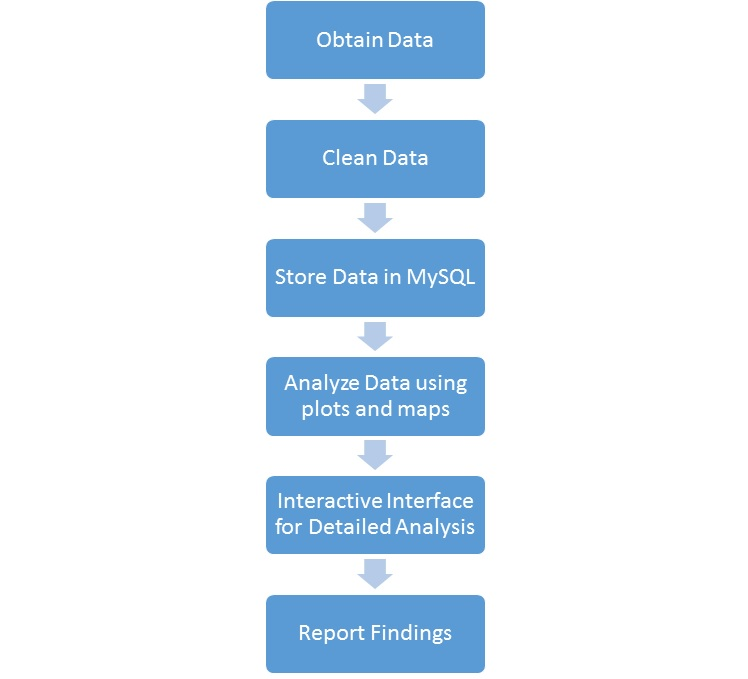
\includegraphics[scale=1.5]{workflow}
  \caption{The project workflow}

\end{figure}


I gathered data from the World Bank’s website for both male and female children out of school from the years 2000 to 2015. I cleaned the data by replacing missing values with the average number of children out of school for a particular country by gender. I then stored the data in a MySQL database. The data was also exported to csv to be used for analysis in R. I did all this in Python. I plotted the graphs and maps from various angles to answer all the research questions. Some of the graphs were made in Python using matplotlib. I then thought an interactive interface would help to analyze the data better. The users will also be able to look at the data from various angles and answer further questions that they may have about the data. The interface was made interactive using R Shiny. The interactive plots and maps were all made using R. The findings were all documented in a report.


\subsection{Project structure}

The data was obtained from the World Bank’s website. Following are the links to the indicators for the male and female children out of primary school.
\begin{itemize}
\item Male Children: \url{http://data.worldbank.org/indicator/SE.PRM.UNER.MA}
\item Female Children: \url{http://data.worldbank.org/indicator/SE.PRM.UNER.FE}
\end{itemize}
The data was in a consistent format. Number of children out of school were listed for all the countries across the year 2000 to 2015. There were some missing values which were replaced by the average number of male/female children out of school for that country.
\subsection{Figures and Tables}

The following graph shows the total male and female children out of primary school from 2000 to 2015.

\begin{figure}[H]
  \centering
    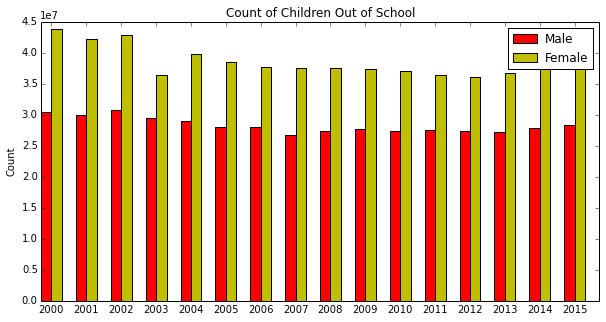
\includegraphics[scale=0.7]{BarTotal}
  \caption{Total counts of male and female children out of primary school 2000-2015}
\end{figure}

The next graph shows the top 10 countries with the maximum number of children out of primary school.
\begin{figure}[H]
  \centering
    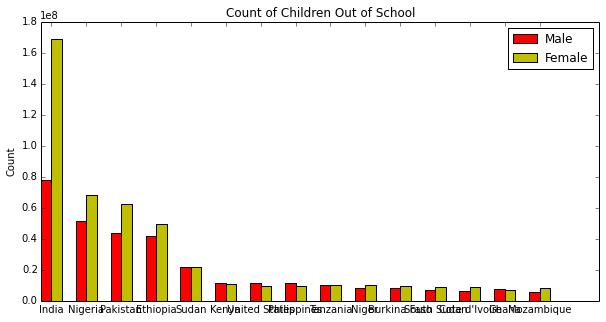
\includegraphics[scale=0.7]{Bar10}
  \caption{Top 10 Countries (Overall)}
\end{figure}

To investigate the top 10 countries in detail, I made an interactive application which helps to select the year for which the data is to be plotted. The following table shows the top 10 countries  that has the most number of children out of primary school in 2015.

\begin{table}[H]
  \centering
    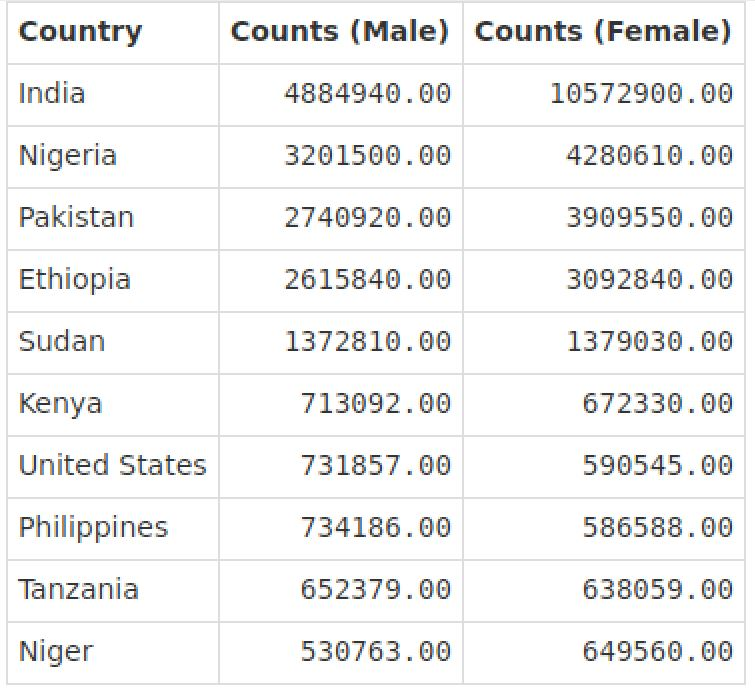
\includegraphics[scale=1]{Top102015}
  \caption{Top 10 Countries (2015)}
\end{table}

A heat map shows the comparison of all the countries for the selected year. Following maps are for male and female children out of school in 2015.

\begin{figure}[H]
  \centering
    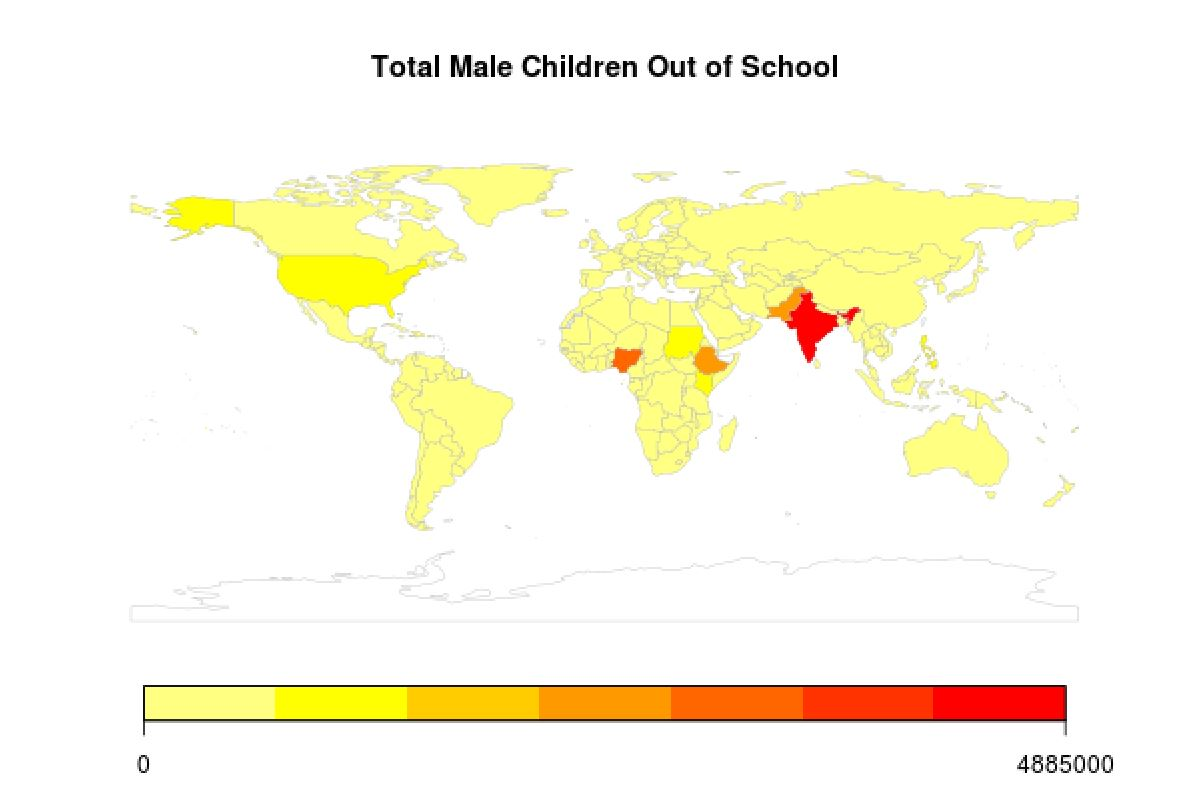
\includegraphics[scale=0.9]{MaleMap}
  \caption{Comparison of all Countries (Male Children, 2015)}
\end{figure}

\begin{figure}[H]
  \centering
    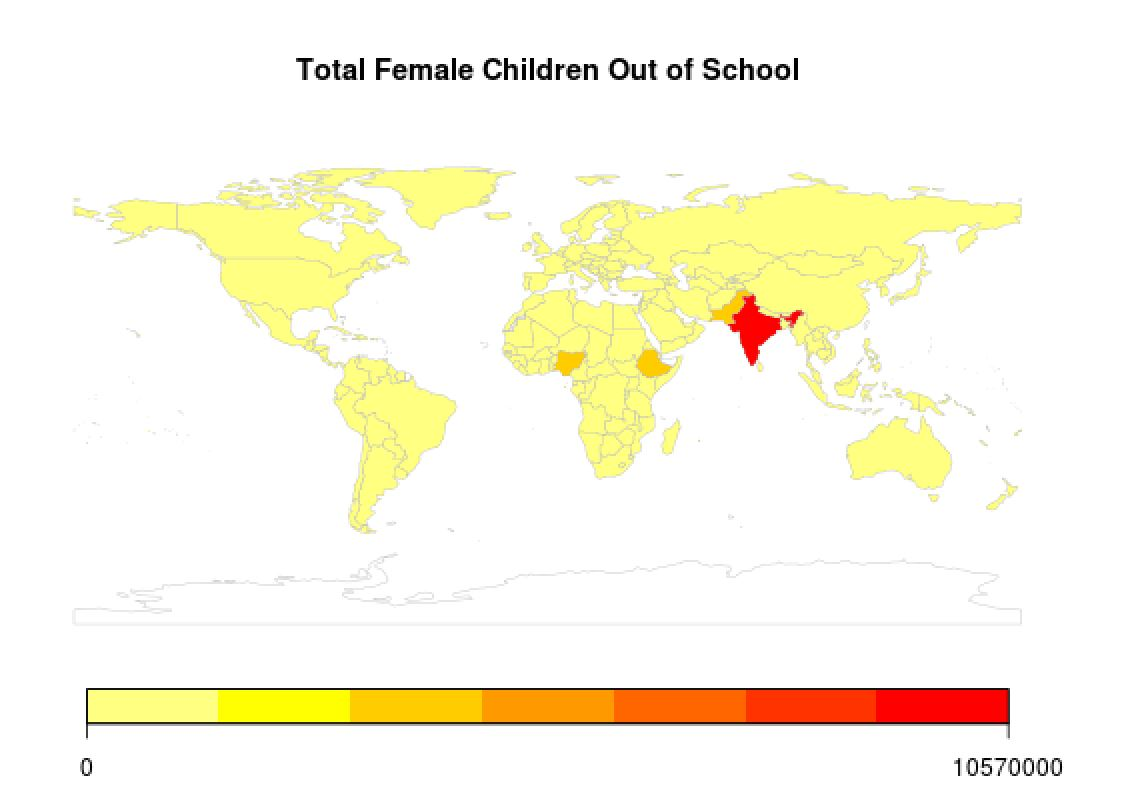
\includegraphics[scale=0.9]{FemaleMap}
  \caption{Comparison of all Countries (Female Children, 2015)}
\end{figure}

The following line charts shows the trend of children out of school for all the countries combined. 

\begin{figure}[H]
  \centering
    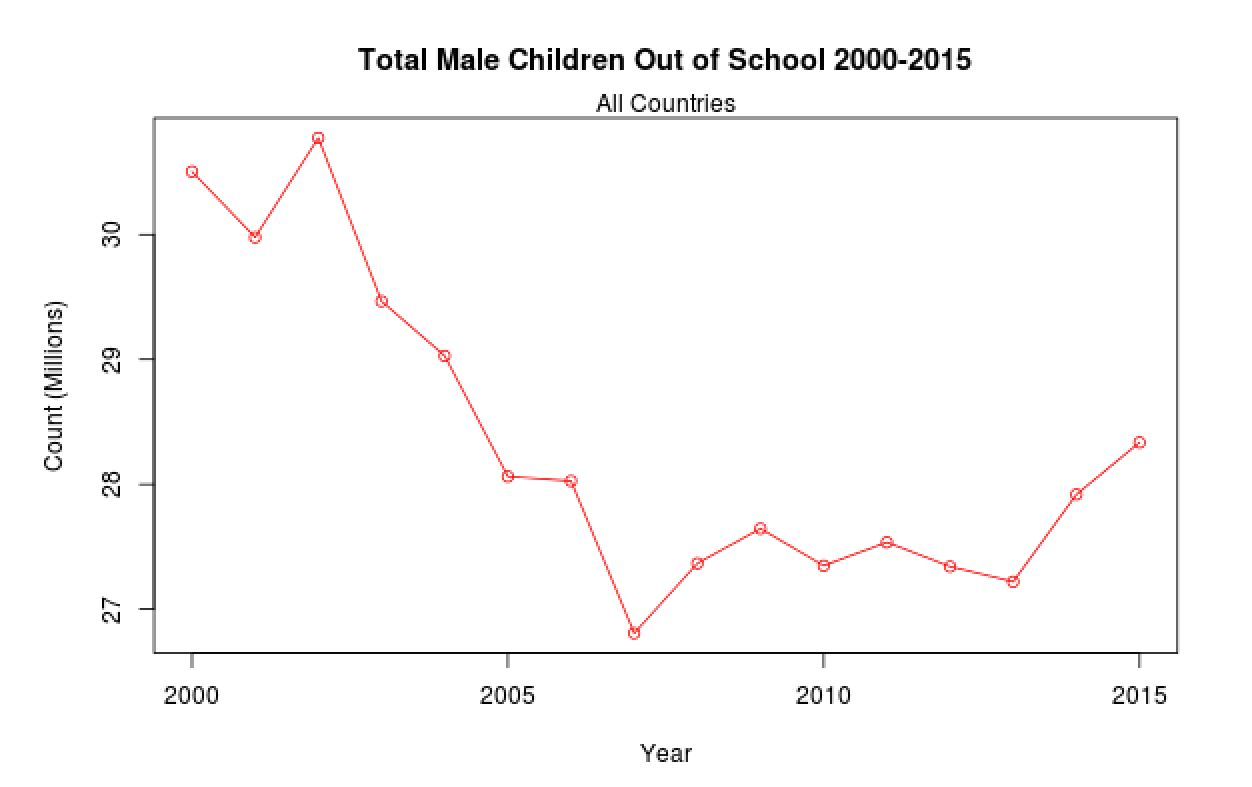
\includegraphics[scale=0.9]{MaleTrendAll}
  \caption{All Countries Trend Male 2000-2015}
\end{figure}

\begin{figure}[H]
  \centering
    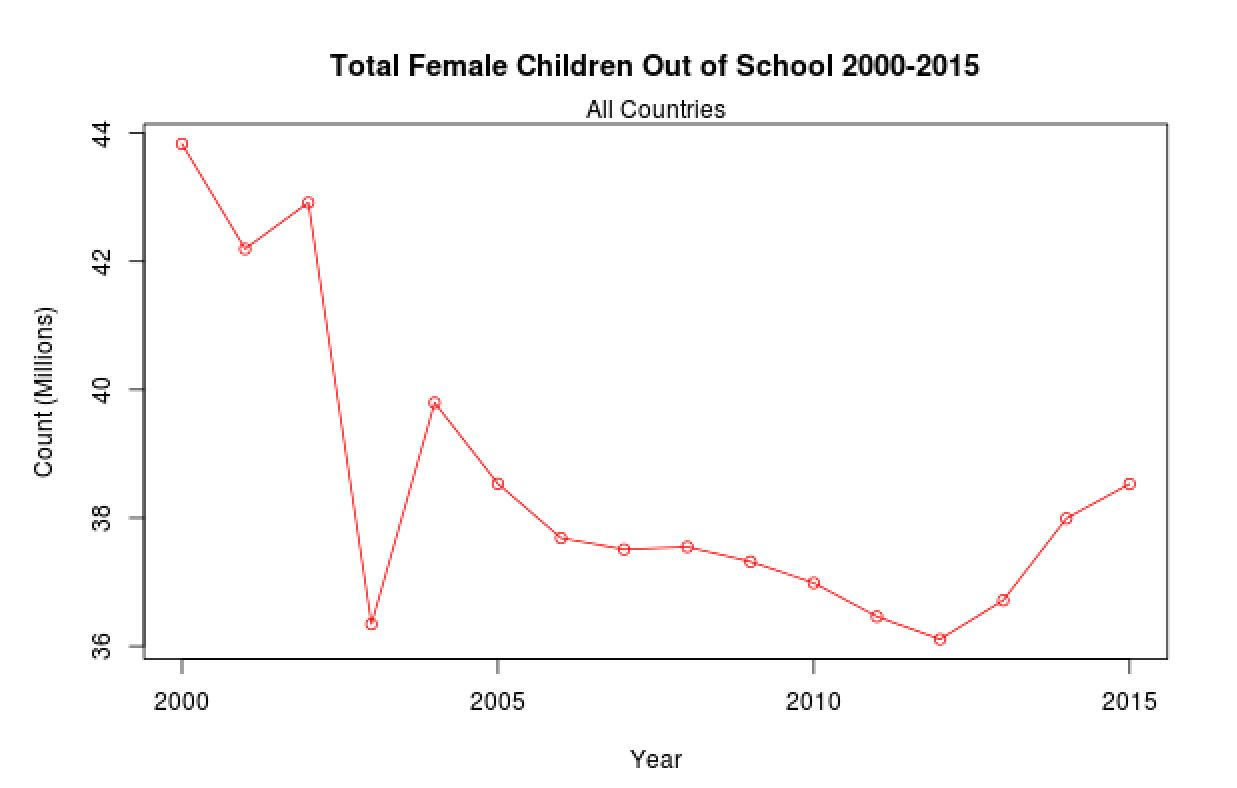
\includegraphics[scale=0.9]{FemaleTrendAll}
  \caption{All Countries Trend Female 2000-2015}
\end{figure}

The interactive user interface also provides an option to look at trends for individual countries. The trend for United States is given below.

\begin{figure}[H]
  \centering
    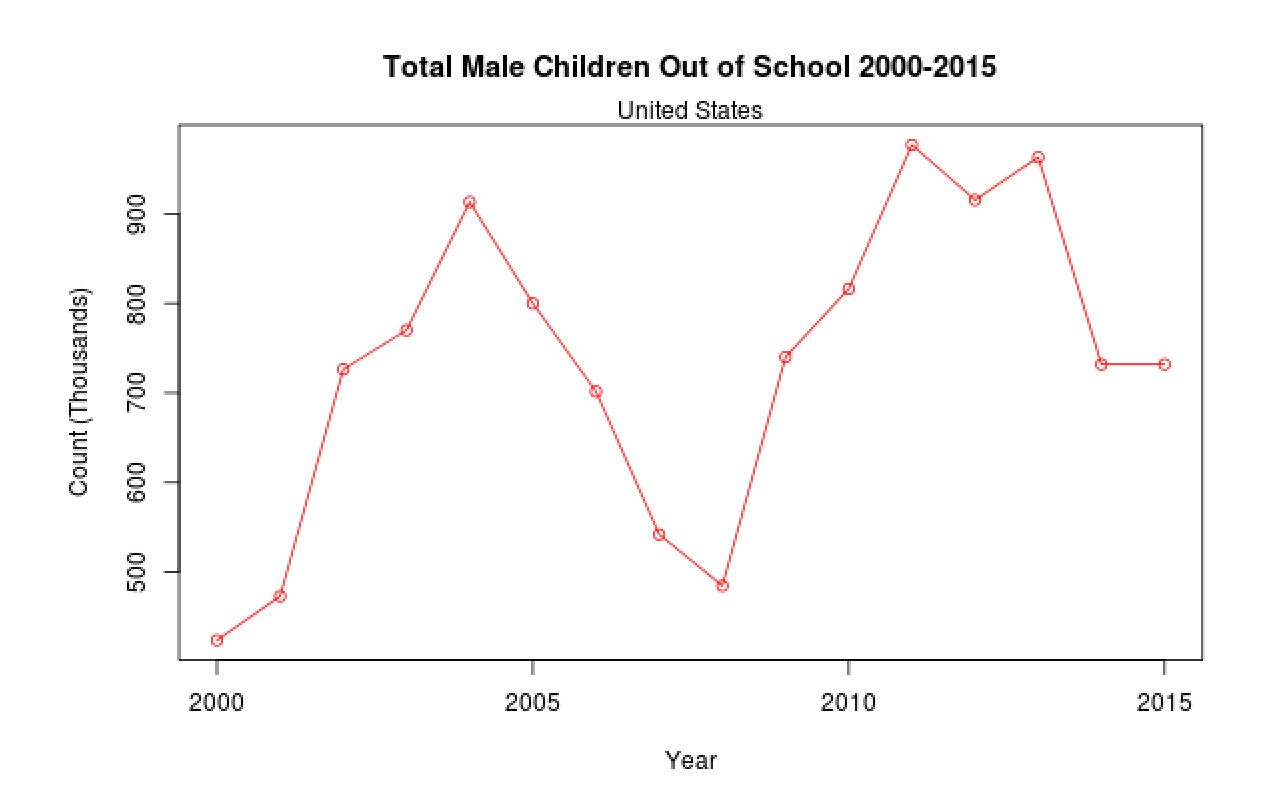
\includegraphics[scale=0.9]{MaleTrendUS}
  \caption{United States Trend Male 2000-2015}
\end{figure}

\begin{figure}[H]
  \centering
    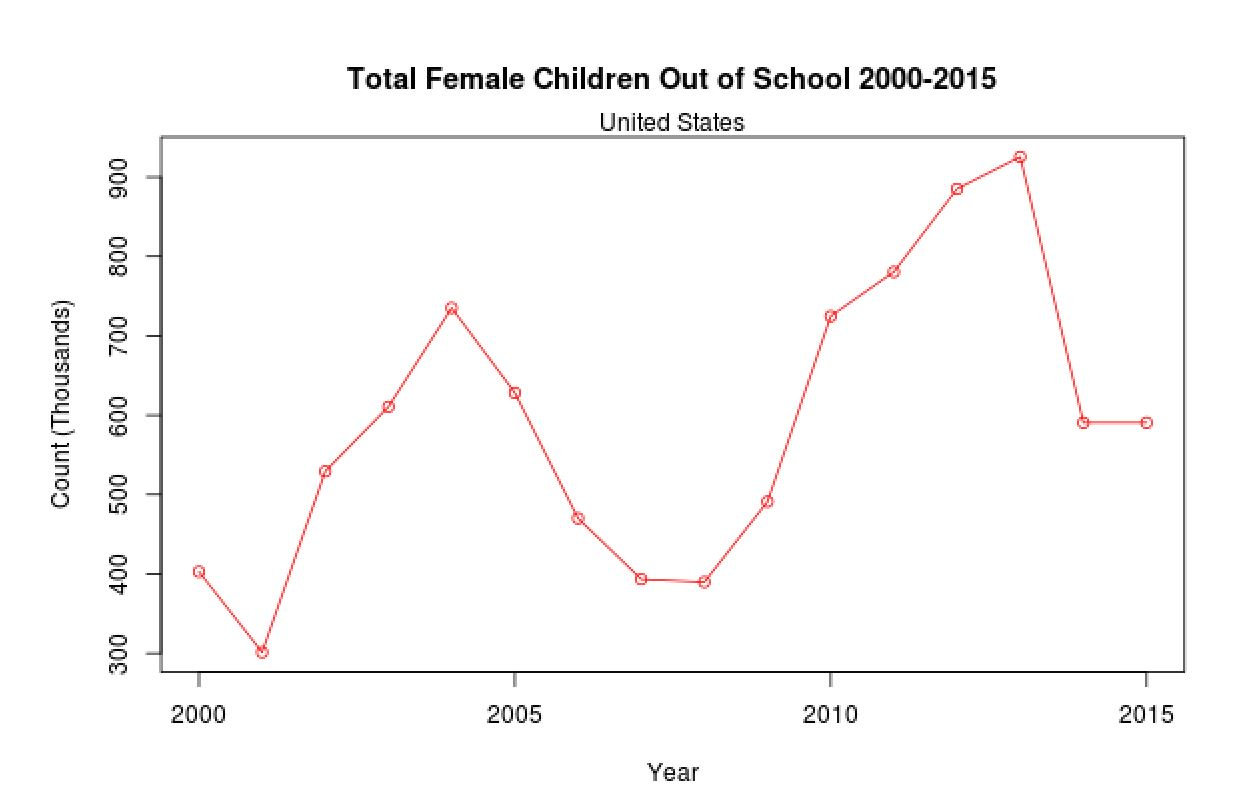
\includegraphics[scale=0.9]{FemaleTrendUS}
  \caption{United States Trend Female 2000-2015}
\end{figure}

\section{Discussion}

The good thing about this project is that it focused on a number of different but related questions about the topic which helped to understand the data better from many angles. It also gives the user an interactive interface which allows the user to play with the data and investigate to answer his own questions. The user might prefer to look at some countries in particular or compare various countries in a particular region. The interactive user interface will allow the user to see the data of his interest in detail.

\subsection{Learnings}

This project required working with data from the web. The data had missing values which gave me a flavor of how the data usually is and how an analyst has to make decisions to deal with missing values in a way that it doesn’t mess up the underlying data or trends. Also, this project required the use of R because of which I made many of the graphs in R. The data was such that I felt the need to have an interactive user interface to look at the data for a particular year or for a particular country. This required making a Shiny app. Because of this project, I experimented with R and played with its code to get my desired graphs and maps which helped me learn R.

\subsection{Challenges}

This project required the use of pandas data frames and R data frames both of which have a huge library of functions available. I needed to look at the data from various angles and I learned how to use both these types of data frames in the process. Making a Shiny application was not a requirement but I felt that the analysis will be more comprehensive if I make an interactive user interface. This helped me in learning Shiny as well.



\section{Conclusion}

The project is a detailed analysis of the number of children out of primary school all over the world from 2000 to 2015. It analyzes the trends over the years, compares all the countries together and highlights the top 10 countries with the largest number of children out of school. It also compares the number of male and female children out of school for all the countries over the time period under observation. The results are interesting to note. India, Nigeria, Pakistan, Ethiopia and United States are in the top 10 list. The number of female children out of school is larger than the number of male children across all the years observed and in all the countries. The project also recommends further study areas for the future.


\end{document}

